\section{User Test}
User Tests are tests that are performed with the help of a group of people that represents a test group from the later end users. The test users have been randomly selected among students in the building. At total of ten students were asked about their opinion of the app. They have been ask to execute the following tasks before filling out a survey about their experience with the app.
\begin{enumerate}
\item select exercise (read description and watch video)
\item learn an exercise (execute exercise ten times with coach)
\item test an exercise (stand alone exercise without help)
\end{enumerate}

These tests should be executed after another. All actions combined represent a typical use case of a user.\\
The tests are only executed with one pair of smartwatch and smartphone since using the second time might influence the opinion of people and their rating of the app.

\subsection{User Test Survey}
The survey should answer the questions listed below.
\begin{itemize}
\item Is the GUI easy to understandable ?
\item is the amount of exercises, their descriptions, videos understandable ?
\item does the app assist the user appropriately ?
\item does user understand the feedback ?
\item is the learning process clear ?
\item does the user have improvements/remarks
\end{itemize}
Since the application was a prototype that lacks the feedback and reliable learning functions, these questions were left out in the survey.
Why these questions ?\\
An app that the user does not understand is not worthy. To make sure the user knows how the app works, it is important to ask wehter the GUI is understandable.
Furthermore it is, from the health point of view, important to make sure that the user does the right movements. That is why the descriptions and videos should be understandable. Another aspect that should be tested is of well the app assists users when doing their exercise compared to exercising without the app.
Given the tester the possibility to make furher remarks for improvements makes it possible for the test user to adress aspects of the app that have not been part of the test.

\subsection{User Test Results}
\begin{figure}[b!]
  \centering
    \begin{minipage}{0.3\textwidth}
      \centering
        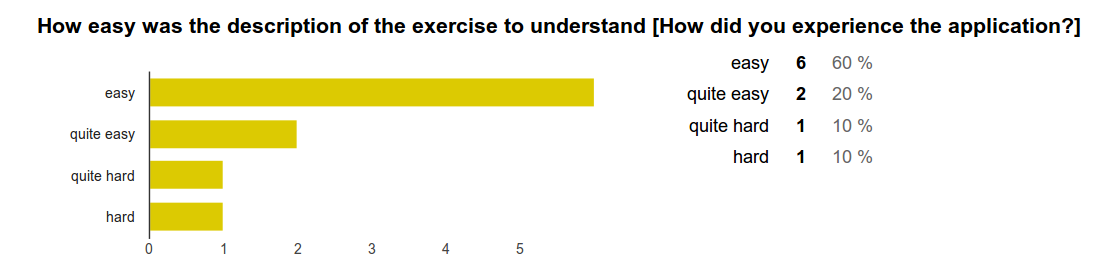
\includegraphics[width=1\textwidth]{00_resources/figures/survey_results4.png}
    \end{minipage}
    \begin{minipage}{0.3\textwidth}
      \centering
        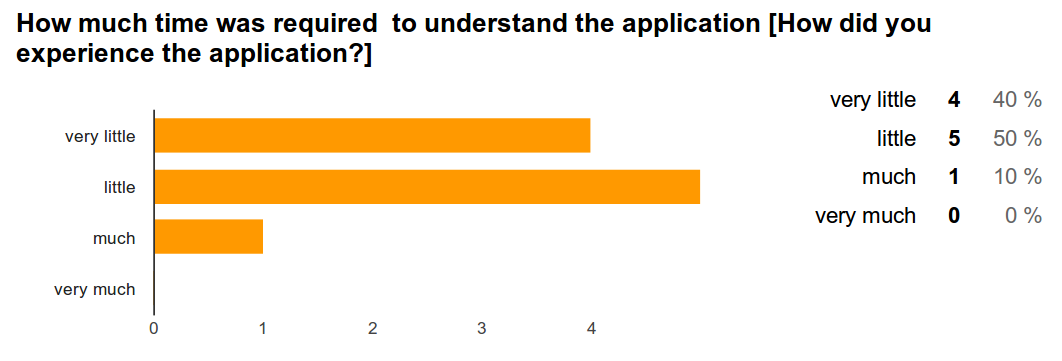
\includegraphics[width=1\textwidth]{00_resources/figures/survey_results5.png}
    \end{minipage}
  \caption{survey results part 2 /2 }
  \label{fig:survey2}
\end{figure}
After anaylzing the survey results, the following conclusions can be drawn. 40 \% tested the pair Samsung Gear S and Samsung Galaxy S, the other 60 \% tested the Sony Smartwatch 3 and the Google Nexus 5.
\\
The application user interface is understandable. 80 \% of the test users agreed that the application was 'easy' or 'quite easy' to understand. Not much time was required to understand the application since 90 \% of the testers needed 'little ' or 'very little' time to understand to understand how the application works. In general the GUI interface of the Samsung Gear S, is more understandable.\\
A little bit harder to understand where the description and the video. For 20 \% of the people the description and video was 'hard' or 'quite hard' to understand. That is the reason why only 60 \% claimed that the app assists them during making the exercises.
\begin{figure}[b!]
  \centering
    \begin{minipage}{0.3\textwidth}
      \centering
        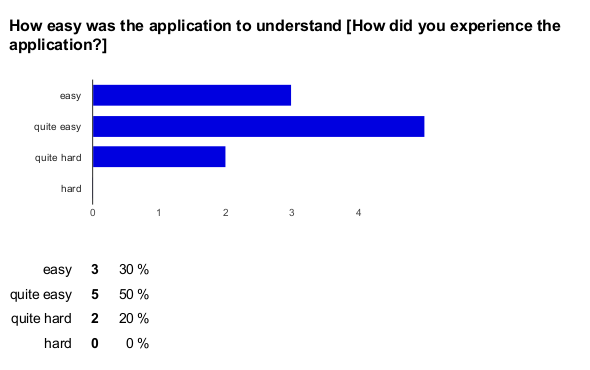
\includegraphics[width=1\textwidth]{00_resources/figures/survey_results1.png}
    \end{minipage}
    \begin{minipage}{0.3\textwidth}
      \centering
        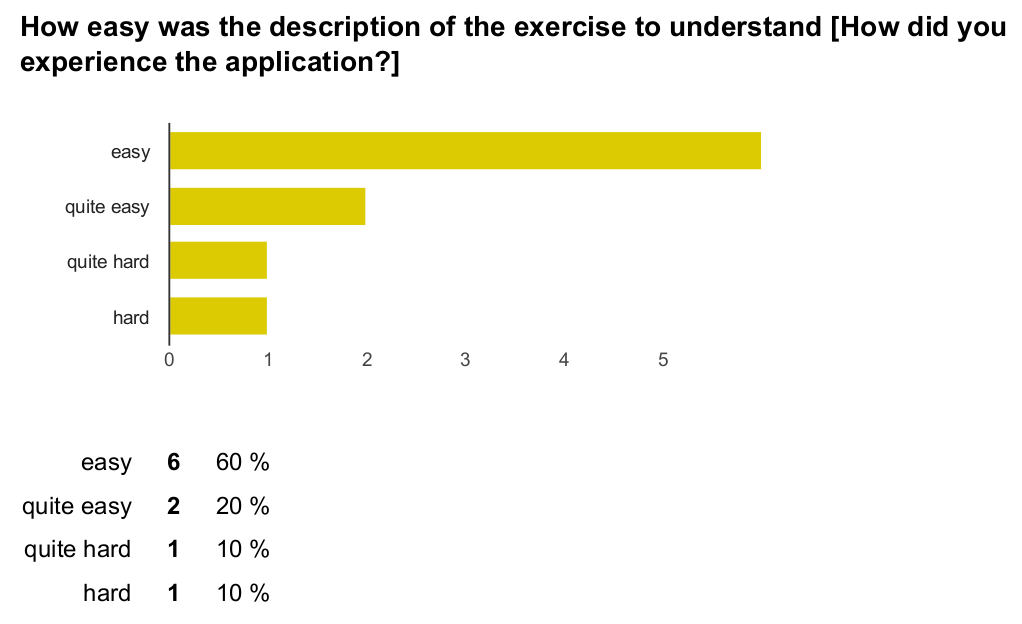
\includegraphics[width=1\textwidth]{00_resources/figures/survey_results2.png}
    \end{minipage}
    \begin{minipage}{0.3\textwidth}
      \centering
        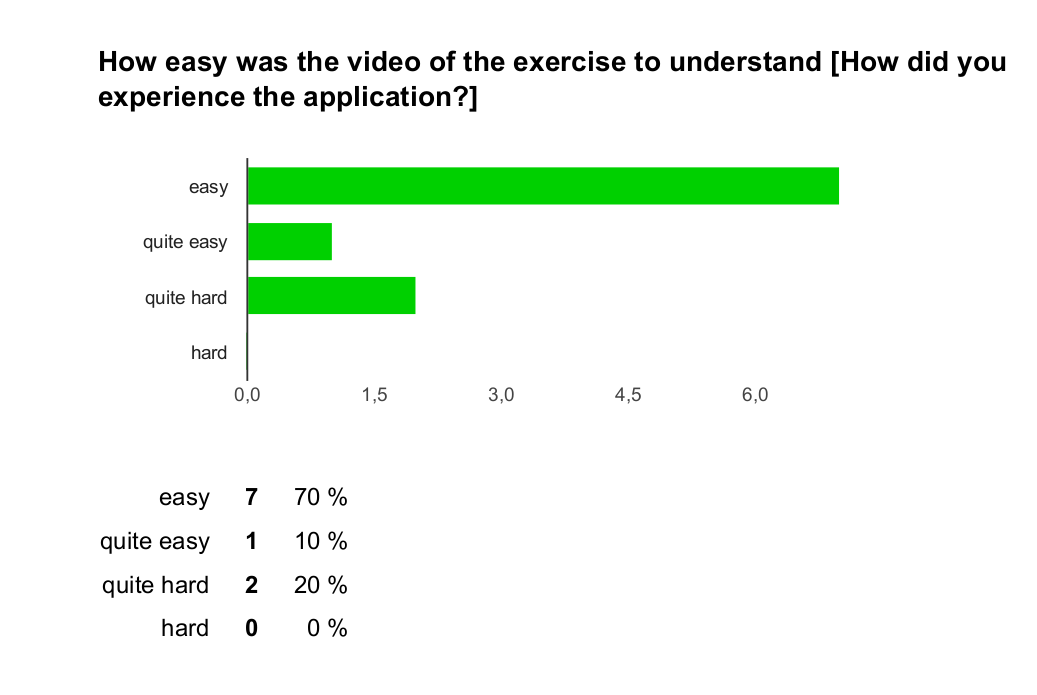
\includegraphics[width=1\textwidth]{00_resources/figures/survey_results3.png}
    \end{minipage}
  \caption{survey results part 1 /2 }
  \label{fig:survey1}
\end{figure}
